\chapter{การเรียนรู้แบบลึก}
\label{chapter: ANN deep learning}

\begin{verse}
``What you get by achieving your goals is not as important as what you become by achieving your goals.'' \\
Johann Wolfgang von Goethe
\end{verse}


%
\begin{figure}
\begin{center}
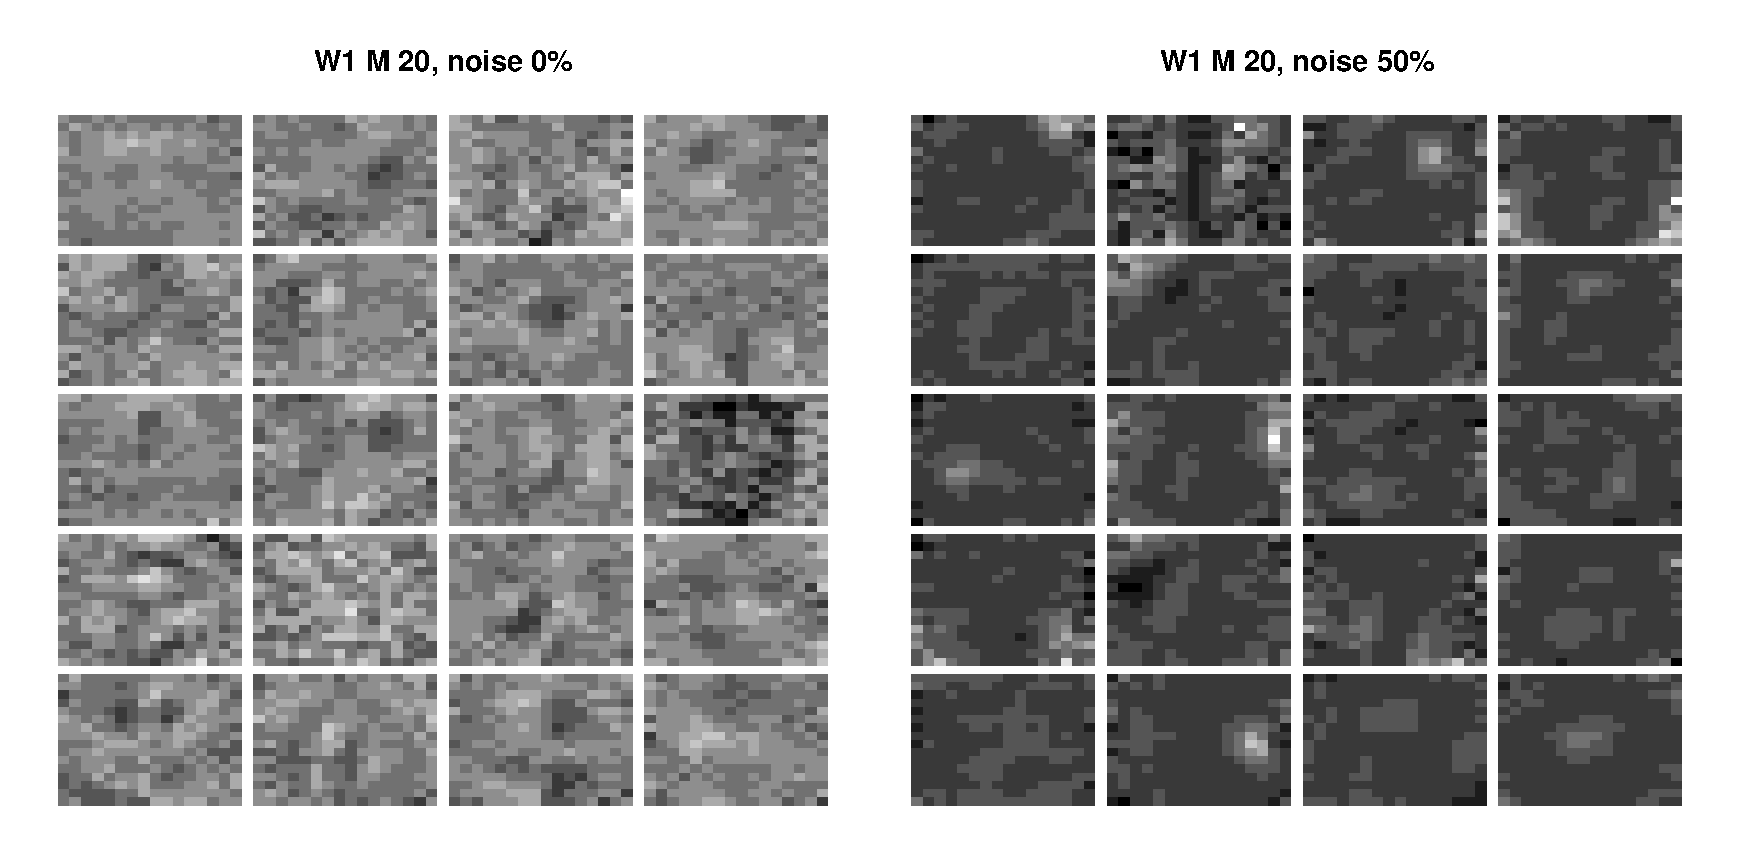
\includegraphics[width=6in]{04ANNDeep/ae01WplotsA.eps}
\end{center}
\caption{autoencoder learned weights with noise M 20}
\label{fig: deep autoencoder learned weights with noise M 20}
\end{figure}
%

%
\begin{figure}
\begin{center}
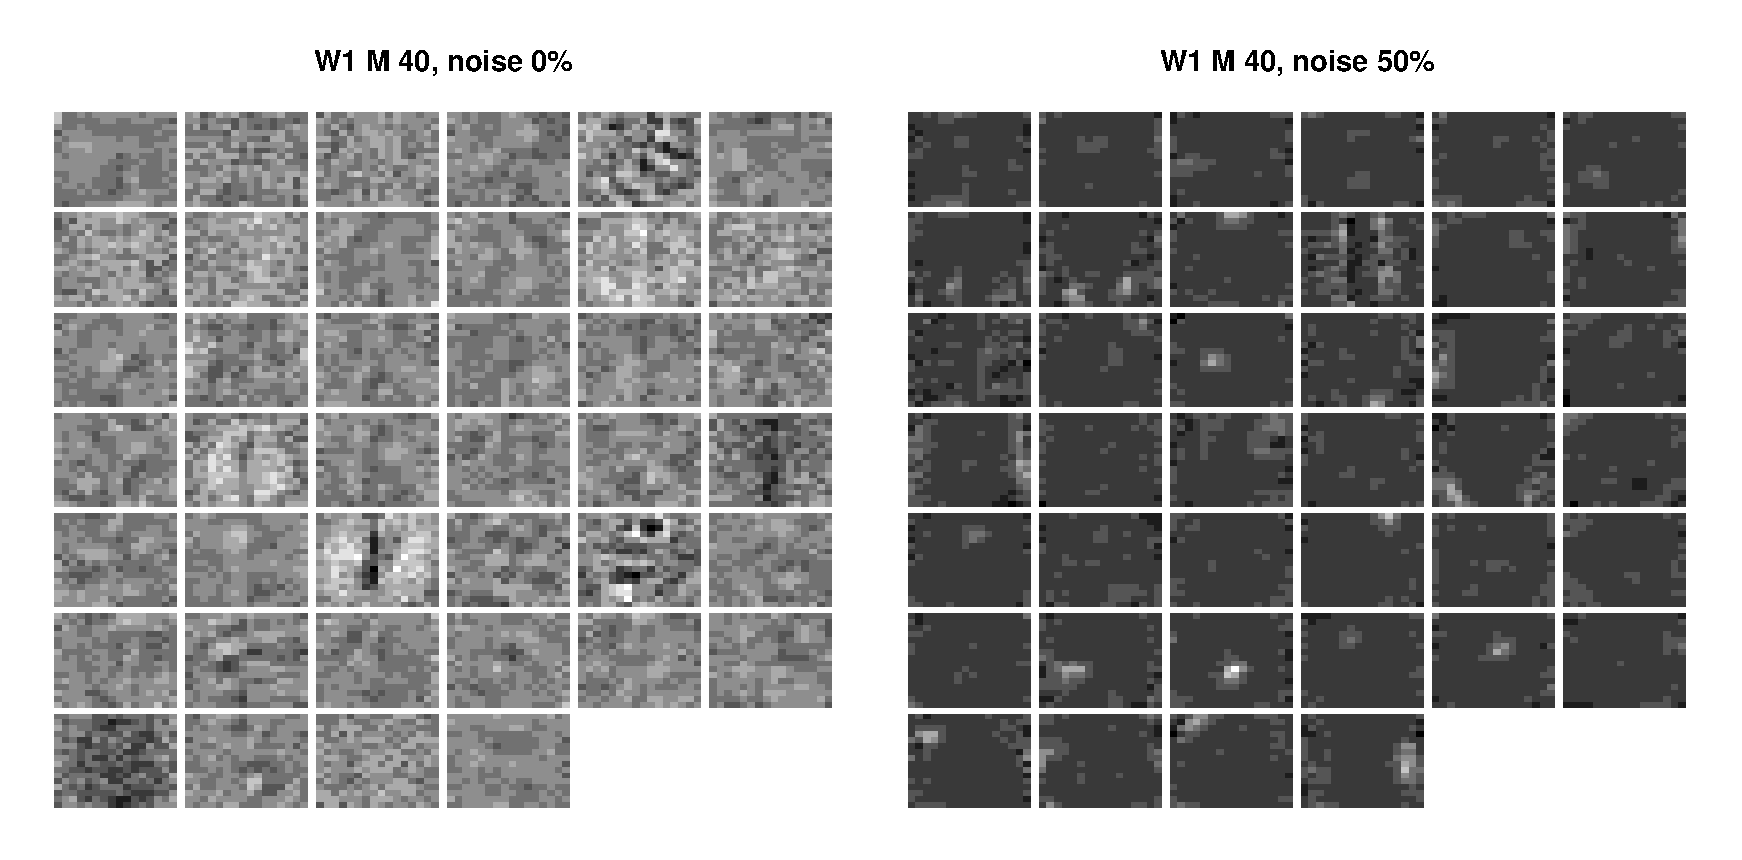
\includegraphics[width=6in]{04ANNDeep/ae01WplotsB.eps}
\end{center}
\caption{autoencoder learned weights with noise M 40}
\label{fig: deep autoencoder learned weights with noise M 40}
\end{figure}
%

%
\begin{figure}
\begin{center}
\includegraphics[width=6in]{04ANNDeep/ae01WplotsC.eps}
\end{center}
\caption{autoencoder learned weights with noise M 256}
\label{fig: deep autoencoder learned weights with noise M 256}
\end{figure}
%

%
\begin{figure}
\begin{center}
\includegraphics[width=6in]{04ANNDeep/ae01WplotsD.eps}
\end{center}
\caption{deep autoencoder learned weights with noise M 500}
\label{fig: deep autoencoder learned weights with noise M 500}
\end{figure}
%

%
\begin{figure}
\begin{center}
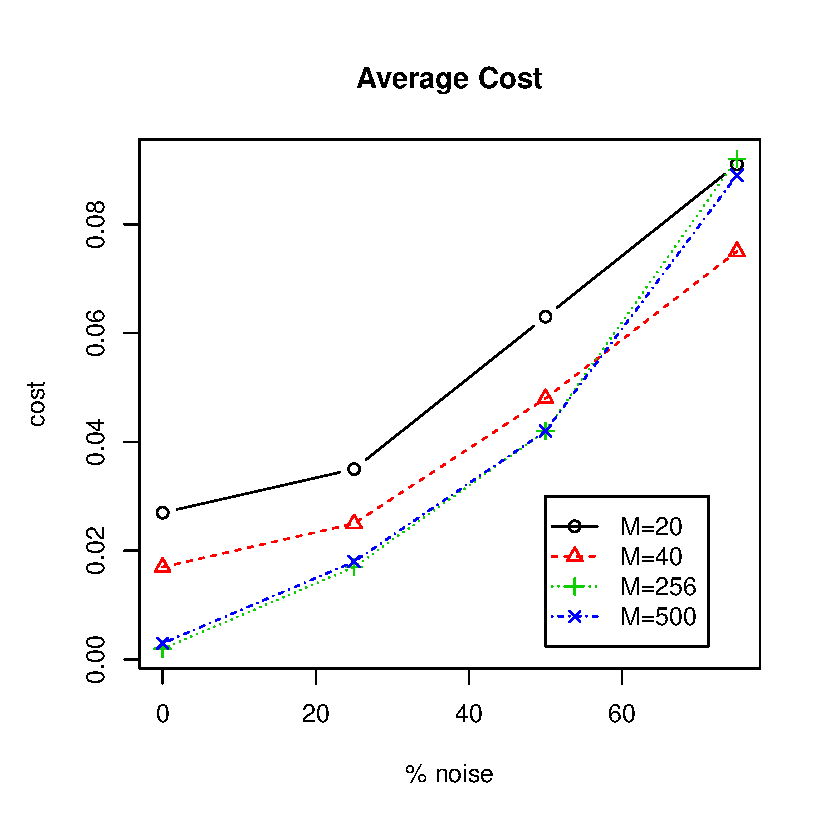
\includegraphics[width=6in]{04ANNDeep/aeReconstructionCostMNoise01.eps}
\end{center}
\caption{autoencoder recontruction costs}
\label{fig: deep autoencoder recontruction costs}
\end{figure}
%

%
\begin{figure}
\begin{center}
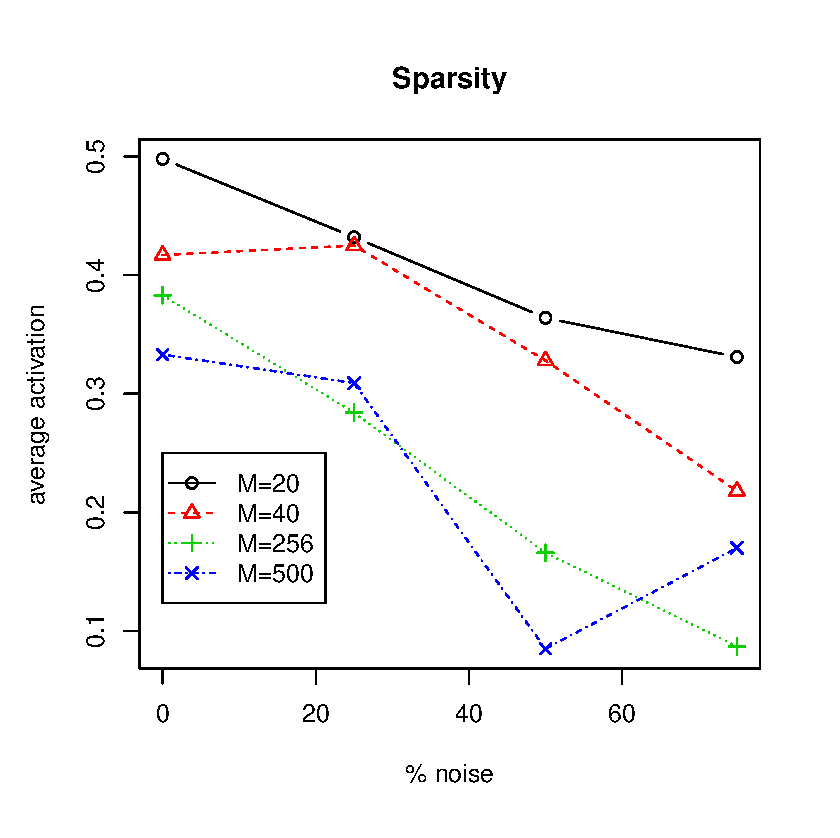
\includegraphics[width=6in]{04ANNDeep/aeSparsityMNoise01.eps}
\end{center}
\caption{autoencoder sparsity}
\label{fig: deep autoencoder sparsity}
\end{figure}
%

%
\begin{figure}
\begin{center}
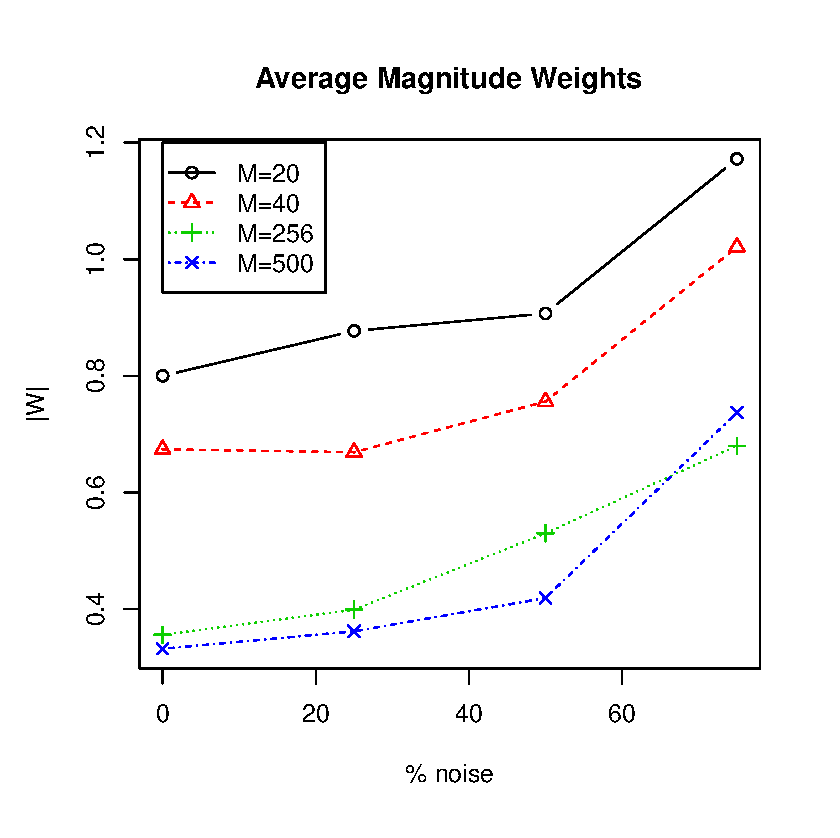
\includegraphics[width=6in]{04ANNDeep/aeWbyMNoise01.eps}
\end{center}
\caption{autoencoder weight magnitude}
\label{fig: deep autoencoder weight magnitude}
\end{figure}
%

%
\begin{figure}
\begin{center}
\includegraphics[width=6in]{04ANNDeep/ae01reconAB.eps}
\end{center}
\caption{deep autoencoder reconstruction samples with noise M 20 and M 40}
\label{fig: deep autoencoder reconstruction samples with noise M 20 and M 40}
\end{figure}
%

%
\begin{figure}
\begin{center}
\includegraphics[width=6in]{04ANNDeep/ae01reconCD.eps}
\end{center}
\caption{deep autoencoder reconstruction samples with noise M 256 and M 500}
\label{fig: deep autoencoder reconstruction samples with noise M 256 and M 500}
\end{figure}
%

จากรูป~\ref{fig: deep autoencoder reconstruction with most activating features M 40 noise 0}, \ref{fig: deep autoencoder reconstruction with most activating features M 40 noise 50}, \ref{fig: deep autoencoder reconstruction with most activating features M 256 noise 0}, และ \ref{fig: deep autoencoder reconstruction with most activating features M 256 noise 50},
สังเกตุว่า การเพิ่มสัญญาณรบกวนเข้าไป นอกจากจะทำให้ ค่าน้ำหนัก W1 แสดง features ได้ชัดเจนขึ้นแล้ว เวลาที่เราทำการ reconstruct กลับ ยังทำให้ได้ลักษณะสำคัญของภาพสมบูรณ์เร็วขึ้นด้วย.

%
\begin{figure}
\begin{center}
\includegraphics[width=6in]{04ANNDeep/ae04aGenEffects.eps}
\end{center}
\caption{autoencoder reconstruction with most activating features M 40 noise 0 เปอร์เซ็นต์}
\label{fig: deep autoencoder reconstruction with most activating features M 40 noise 0}
\end{figure}
%

%
\begin{figure}
\begin{center}
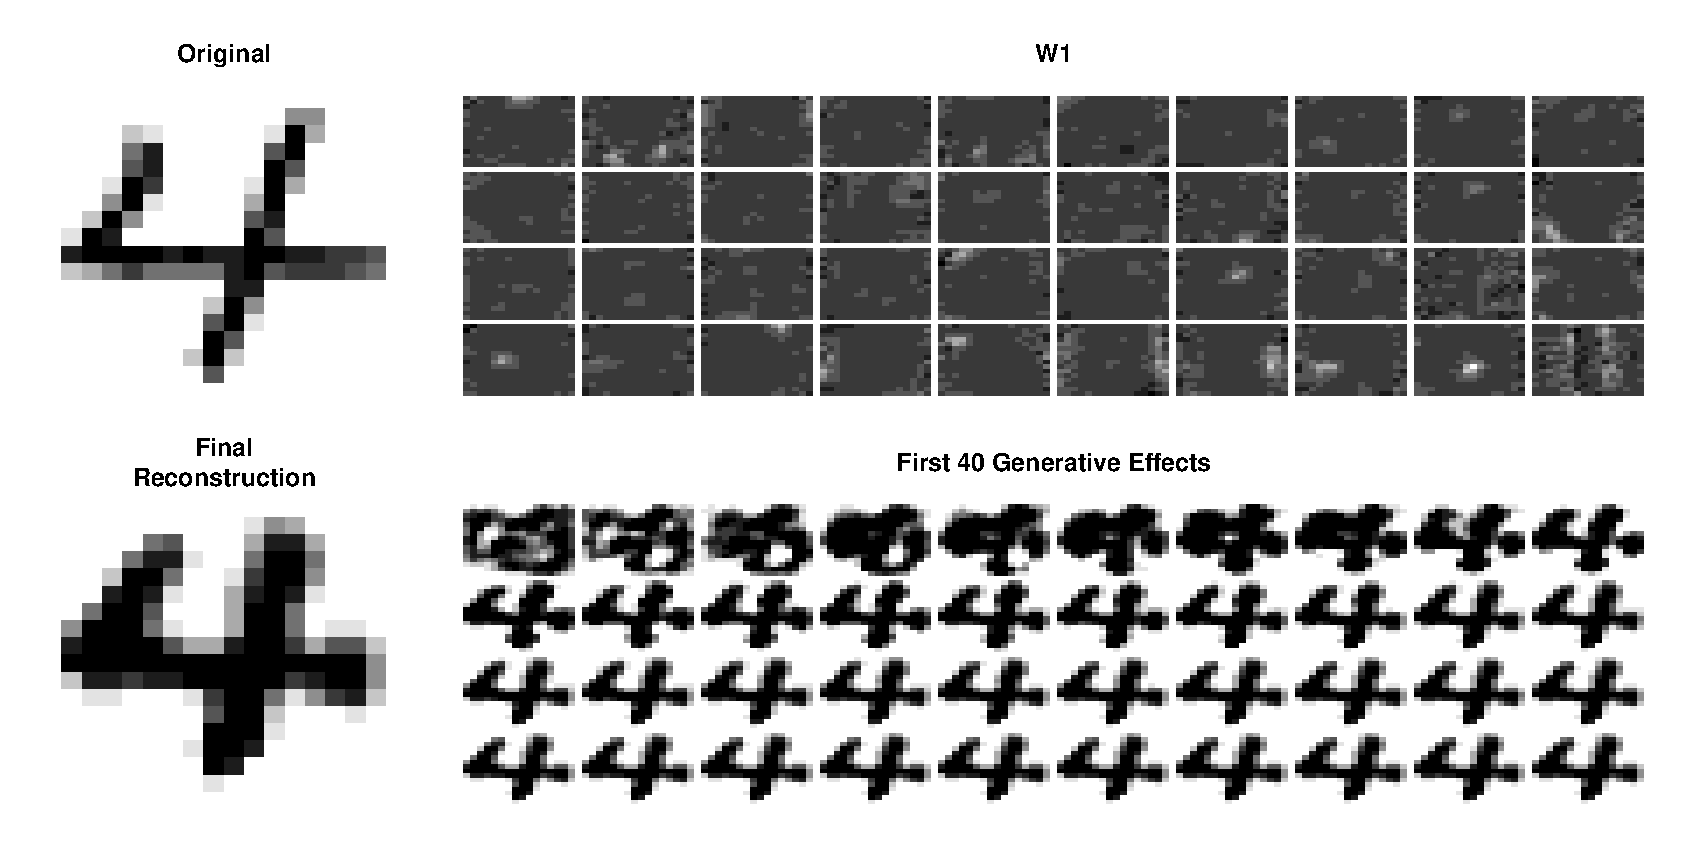
\includegraphics[width=6in]{04ANNDeep/ae04cGenEffects.eps}
\end{center}
\caption{autoencoder reconstruction with most activating features M 40 noise 50 เปอร์เซ็นต์}
\label{fig: deep autoencoder reconstruction with most activating features M 40 noise 50}
\end{figure}
%

%
\begin{figure}
\begin{center}
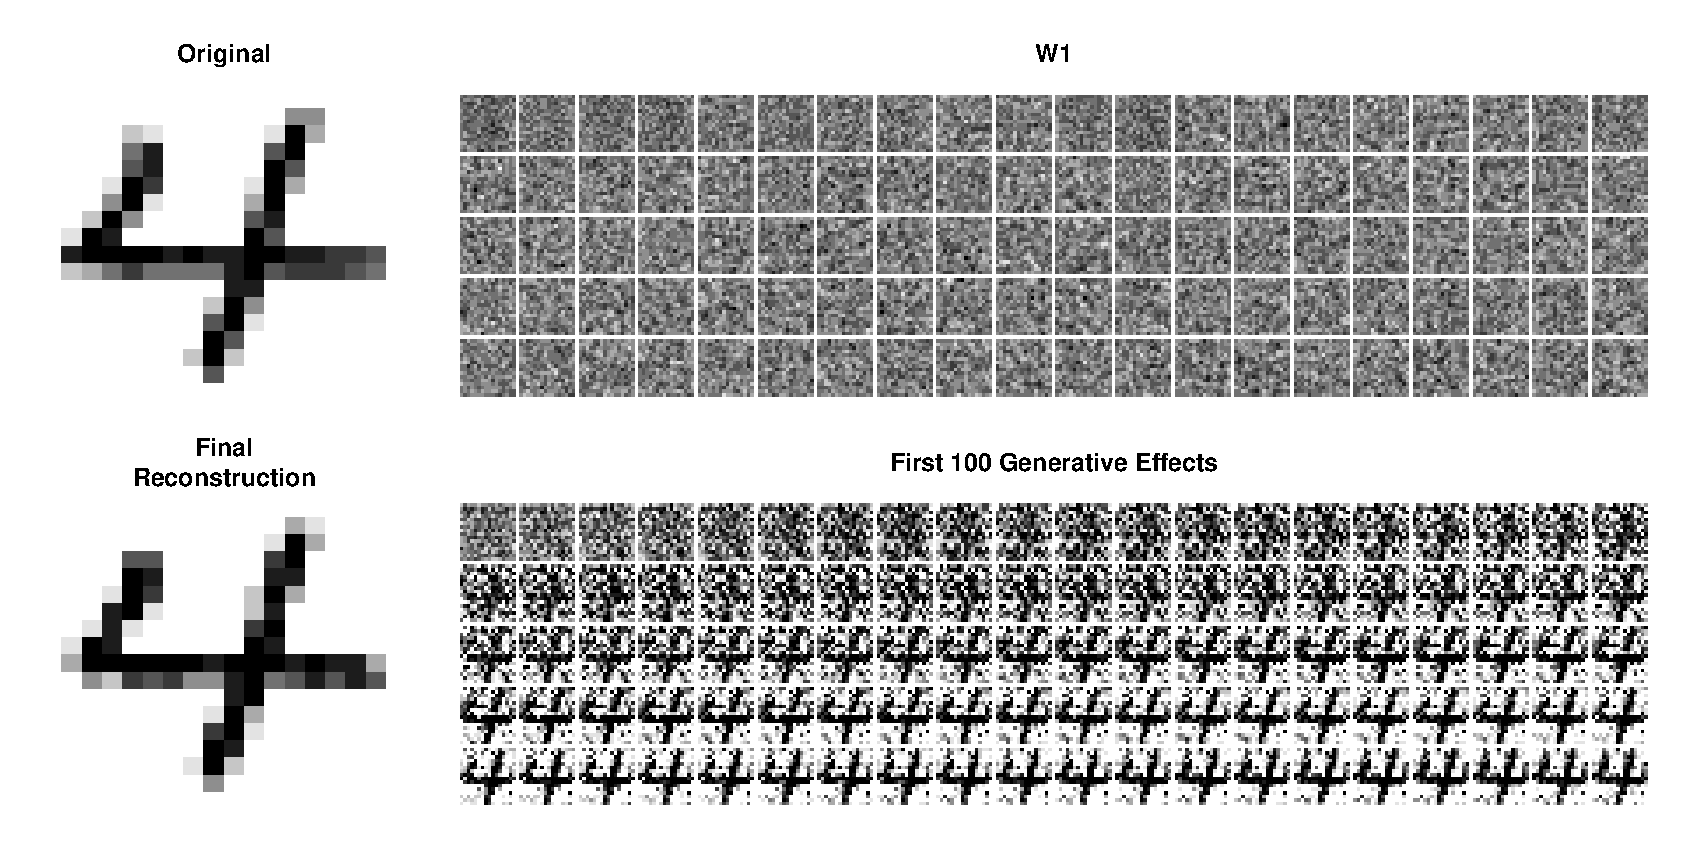
\includegraphics[width=6in]{04ANNDeep/ae06aGenEffects.eps}
\end{center}
\caption{autoencoder reconstruction with most activating features M 500 noise 0 เปอร์เซ็นต์}
\label{fig: deep autoencoder reconstruction with most activating features M 500 noise 0}
\end{figure}
%

%
\begin{figure}
\begin{center}
\includegraphics[width=6in]{04ANNDeep/ae06cGenEffects.eps}
\end{center}
\caption{autoencoder reconstruction with most activating features M 500 noise 50 เปอร์เซ็นต์}
\label{fig: deep autoencoder reconstruction with most activating features M 500 noise 0}
\end{figure}
%

\subsection{Sparse Autoencoder}

จาก \cite{ufldl} (Autoencoders and Sparsity), การกระตุ้นเฉลี่ย ของแต่ละหน่วยซ่อน (ของชั้นที่ 1) สามารถวัดได้จาก
\begin{eqnarray}
 \hat{\rho}_m &=& \frac{1}{N} \sum_{n=1}^N h \left( 
w^{(1)}_{m,0} + \sum_{d=1}^D w^{(1)}_{m,d} \cdot x_{d,n} \right)
 \nonumber \\ 
&=& \frac{1}{N} \sum_{n=1}^N h \left( 
 \vec{w}^T_m
  \cdot \begin{bmatrix}
 1 \\
 \vec{x}_n
 \end{bmatrix} \right)
 \nonumber \\ 
&=& \frac{1}{N} \sum_{n=1}^N z_{m,n}
 \nonumber \\  
\label{eq: deep sparse rhohat} 
\end{eqnarray}

เราควบคุมให้ค่าการกระตุ้นเฉลี่ยใกล้เคียงกับค่าเป้าหมาย $\rho$ ได้โดย
\begin{eqnarray}
 \mathrm{Cost} = \mathrm{Cost}_{\mathrm{recon}} 
  + \beta \sum_{m=1}^M \rho \log \frac{\rho}{\hat{\rho}_m} + (1 - \rho) \log \frac{1 - \rho}{1 - \hat{\rho}_m}
\label{eq: deep sparsity cost}  
\end{eqnarray}
เมื่อ $\mathrm{Cost}_{\mathrm{recon}}$ แทน recontruction cost (ค่า cost ในสมการ~\ref{eq: ann cost fn biclass}\footnote{สำหรับอินพุตที่มีค่าอยู่ระหว่าง $[0,1]$.}).
เทอม $\rho \log \frac{\rho}{\hat{\rho}_m} + (1 - \rho) \log \frac{1 - \rho}{1 - \hat{\rho}_m}$ นี้ว่า Kullback-Leibler (KL) divergence\footnote{ทฤษฎีความน่าจะเป็น และ ทฤษฎีสารสนเทศ จะเรียก 
รายละเอียดเกี่ยวกับ KL เทอม ศึกษาเพิ่มเติมได้จาก \cite{KullbackLeibler1951a}.
}.
เทอม KL จะใช้วัดความต่างระหว่างการกระจายความน่าจะเป็นของสองค่า $\rho$ กับ $\hat{\rho}_m$.
รูป .. แสดงค่า KL ที่ค่า $\rho$ และ $\hat{\rho}_m$ ต่างๆ. 
ค่า KL จะเป็น $0$ เมื่อ $\rho = \hat{\rho}_m$ และ ค่า KL มีค่ามาก เมื่อ ค่า $\rho$ และ $\hat{\rho}_m$ ต่างกันมาก.

เมื่อหาค่าอนุพันธ์ ของสมการ~\ref{eq: deep sparsity cost} 
แล้วจะพบว่า เรายังสามารถคำนวณค่าเกรเดียนต์ ด้วยวิธีการแพร่กระจายย้อยกลับ
เมื่อรวมเงื่อนไขบังคับ sparsity เพียงแต่ดัดแปลง สมการ~\ref{eq: ANN BP delta j} ให้เป็น
\begin{eqnarray}
  \delta_j &=& h'(a_j) \left( \sum_k w_{kj} \delta_k + \beta \left( -\frac{\rho}{\hat{\rho}_j} + \frac{1 - \rho}{1 - \hat{\rho}_j} \right) \right)
\nonumber \\
&=& h'(a_j) \sum_k w_{kj} \delta_k + \beta \cdot h'(a_j) \left( -\frac{\rho}{\hat{\rho}_j} + \frac{1 - \rho}{1 - \hat{\rho}_j} \right)
\label{eq: deep BP delta j sparsity}
\end{eqnarray}
เท่านั้น.
% 


%
\begin{figure}
\begin{center}
\includegraphics[width=6in]{04ANNDeep/KL01.eps}
\end{center}
\caption{Kullback-Liebler term ที่ค่าเปรียบเทียบต่างๆ}
\label{fig: deep KL characteristics}
\end{figure}
%



``The restricted Boltzmann machine has been the subject of a recent resurgence of interest due to its role as the building block of the deep belief network. Deep belief networks are designed to learn feature hierarchies to automatically find high-level representations for high-dimensional data. A deep belief network comprises a stack of restricted Boltzmann machines. Given a piece of data (state of the lowest visible variables), each layer's most likely hidden states are treated as data for the next layer. A new effective train methodology for deep belief networks, which begins by training each layer in turn as an RBM using contrastive divergence, was introduced by Hinton et al. \cite{HintonEtAl2006a}. This method led to many new applications in general machine learning problems including object recognition and dimensionality reduction \cite{HintonSalakhutdinov2006a}. ... 
Le Roux and Bengio \cite{LeRouxBengio2008a} showed that any distribution with support on $r$ visible states may be arbitrarilt well approximated provided there are at least $r+1$ hidden nodes.
Therefore, any distribution can be approximated with $2^n + 1$ hidden nodes [$n$ is a number of observed variables].

Therefore any distribution can  '' \cite{CuetoEtAl2009a}

``The central hypothesis is that good feature sets contain features that are highly correlated
with the class, yet uncorrelated with each other.'' from Hall, M. A., Correlation-based Feature Selection for Machine Learning, Ph.D. Thesis, Department of Computer Science, University of Waikato, New Zealand, 1999


``One of the main purposes of unsupervised learning is to produce good representation for data, that can be used for detection, recognition, prediction, or visualization. Good representation eliminate irrelevant variabilities of the input data, while preserving the information that is useful for the ultimate task.''
Marc'Aurelio Ranzato, Y-Lan Boureau, Yann LeCun, "Sparse Feature Learning for Deep Belief Networks", 